
\documentclass[runningheads]{llncs}
%
\renewcommand{\figurename}{Figure}

\usepackage[T1]{fontenc}
\usepackage{comment}
\usepackage{graphicx}
\usepackage{amsmath}
\usepackage{float}
\usepackage{multirow}
\usepackage{multicol}
\usepackage{marvosym}
\usepackage{ifsym}
\usepackage{amssymb}

\usepackage[table]{xcolor}
\usepackage[autostyle=false, style=english]{csquotes}\MakeOuterQuote{"}

\renewcommand{\arraystretch}{1.25}

\begin{document}
%
\title{Title}
%
\titlerunning{Title}
% If the paper title is too long for the running head, you can set
% an abbreviated paper title here
%
% \author{Nguyen Xuan Thanh\inst{1,2} \and
% Le Duc Hoang Nam\inst{1,2} \and
% Quang Tran Minh\inst{1,2} \and 
% Trong Nhan Phan\inst{1,2}\thanks{Corresponding author.}}
\author{Author1\inst{1,2} \and 
Author2\inst{1,2}\textsuperscript{\Letter}}
%
\authorrunning{Vo et al.}
\institute{Faculty of Computer Science and Engineering, Ho Chi Minh City University of Technology (HCMUT), 268 Ly Thuong Kiet, District 10, Ho Chi Minh City, Vietnam.\\
\and
Vietnam National University Ho Chi Minh City (VNU-HCM), Linh Trung Ward, Thu Duc District, Ho Chi Minh City, Vietnam.
\\
\email{\{author1, author2\}@hcmut.edu.vn}}
%
\maketitle              % typeset the header of the contribution
%
\begin{abstract}
<summarize problems and results, 14 to 16 lines>. 


\keywords{lakehouse, framework, healthcare <5-7 keywords>}
\end{abstract}
%
%
%
\section{Introduction}\label{sec1}

<Problem statement, motivation, how problem solved today, any pros and cons, 1 page>.

<summarize contribution>. Our main contributions include the followings: 
\begin{itemize}
    \item Tbc.
    \item Tbc.
    \item Tbc.
\end{itemize}

The rest of the paper is organized as follows. Section \ref{sec2} introduces related work. Section \ref{sec3} proposes the architecture and workflow. Section \ref{sec4} evaluates its effectiveness via experiments. Finally, Section \ref{sec5} concludes the paper.

%==============================================%
\section{Related Work}\label{sec2}

<analyze pros and cons of related work, show how different from our work, emphasize the strong points or innovation in our proposed method, 2 pages>
% Background Knowledge
\section{Proposed Method}\label{sec3}
\subsection{Framework}

<describe framework architecture and related flows with figures>. 
biomedclip + cbam
\begin{figure}[!ht]
    \centering    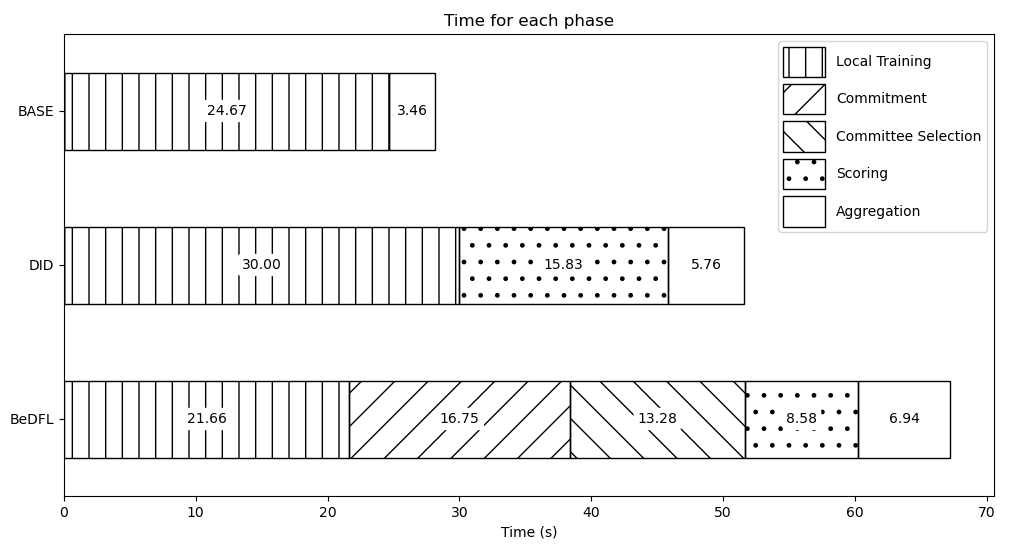
\includegraphics[width=0.6\textheight]{figures/time.png}
    \caption{General System Architecture.}
    \label{fig:architecture_0}
    %\vspace*{-5mm}
\end{figure}

\subsection{Workflow} \label{wf}
<describe related workflows with figures>. 

%------------------------------%
\subsection{Tbc} \label{tbc}
<Any more subsections>.


%==============================================%
\section{Experiments and Analysis}\label{sec4}

\subsection{Environment Settings}\label{exp1}

\textbf{RSNA 2024 LumbarDISC.} About 2{,}000 patients with sagittal T2 stacks. We use a patient-level 80/20 train/validation split (\verb|random_state = 42|), which gives 1{,}942 validation IVDs from 395 patients. Labels span 5 levels $\times$ 5 conditions $\times$ 3 severities. We restrict evaluation to three of the five conditions (canal stenosis, left and right neural foraminal narrowing) for which sagittal-only input is most clinically appropriate; left and right subarticular stenosis, which are best read on axial reformats, are left to future work. The class distribution per evaluated condition averages Normal/Mild $\approx 85\%$, Moderate $\approx 10\%$, and Severe $\approx 5\%$.

\textbf{SPIDER.}~\cite{vandergraaf2024spider} About 1{,}400 IVDs from 218 patients across four Dutch hospitals (T1 and T2-FS sagittal sequences). For consistency with the RSNA-trained encoder we use the T2-FS sagittal series only. The label schema differs from RSNA: Pfirrmann grades 1--5~\cite{pfirrmann2001}, Modic changes 0--3 (4 classes)~\cite{modic1988}, spondylolisthesis, disc herniation, disc narrowing, disc bulging, and upper/lower endplate damage (all binary). SPIDER is used for cross-dataset evaluation only; no SPIDER image is seen during RSNA training.

Figure~\ref{fig:dist} reports the class distribution of both datasets: the RSNA Severe class stays under 5\%, and several SPIDER labels are similarly skewed. This imbalance is the central difficulty the training pipeline must handle.

\begin{figure}[t]
\centering
\begin{minipage}[t]{0.49\linewidth}
\centering

\includegraphics[width=\linewidth]{rsna_class_distribution.png}\\[1pt]
{\scriptsize (a) RSNA 2024 severity distribution}
\end{minipage}\hfill
\begin{minipage}[t]{0.49\linewidth}
\centering

\includegraphics[width=\linewidth]{spider_class_distribution.png}\\[1pt]
{\scriptsize (b) SPIDER label distribution}
\end{minipage}
\caption{Class distribution of the two datasets. (a) RSNA 2024 per-condition severity, where Normal/Mild dominates and Severe stays under 5\%. (b) SPIDER eight-label distribution, where several pathology labels are heavily skewed toward the negative class.}
\label{fig:dist}
\end{figure}

\textbf{Evaluation metrics.} We report macro-averaged Recall, Precision, F1, AUC (one-vs-rest), and AUPRC, plus per-class Severe metrics. Macro averaging over the $C = 3$ severities, $\frac{1}{C}\sum_{c}\mathrm{metric}_c$, keeps the dominant Normal/Mild class (85\% prevalence) from masking failure on the Severe class. We report AUPRC next to AUC because, on heavily imbalanced data, AUC can stay high while a model fails to rank Severe cases meaningfully; the AUPRC random baseline equals the positive-class prevalence (about 0.05 for Severe).

\textbf{Hardware.} All runs use a single NVIDIA RTX 4090 (Vast.ai), with peak memory of 16\,GB and a cost of roughly \$2 per hybrid run.

\subsection{Empirical Experiments}\label{exp2}
<Describe, analyze, and discuss with figures and tables...>


%==============================================%
\section{Summary}\label{sec5}
<summary and future work, 16 lines>.

\begin{credits}
\subsubsection{\ackname} We acknowledge Ho Chi Minh City University of Technology (HCMUT), VNU-HCM for supporting this study.

% \subsubsection{\discintname}
% It is now necessary to declare any competing interests or to specifically
% state that the authors have no competing interests. Please place the
% statement with a bold run-in heading in small font size beneath the
% (optional) acknowledgments\footnote{If EquinOCS, our proceedings submission
% system, is used, then the disclaimer can be provided directly in the system.},
% for example: The authors have no competing interests to declare that are
% relevant to the content of this article. Or: Author A has received research
% grants from Company W. Author B has received a speaker honorarium from
% Company X and owns stock in Company Y. Author C is a member of committee Z. 
\end{credits}
%
% ---- Bibliography ----
%
% BibTeX users should specify bibliography style 'splncs04'.
% References will then be sorted and formatted in the correct style.
%
\bibliographystyle{splncs04}
\bibliography{references}
%
% \begin{thebibliography}{8}
% \bibitem{ref_article1}
% Author, F.: Article title. Journal \textbf{2}(5), 99--110 (2016)

% \bibitem{ref_lncs1}
% Author, F., Author, S.: Title of a proceedings paper. In: Editor,
% F., Editor, S. (eds.) CONFERENCE 2016, LNCS, vol. 9999, pp. 1--13.
% Springer, Heidelberg (2016). \doi{10.10007/1234567890}

% \bibitem{ref_book1}
% Author, F., Author, S., Author, T.: Book title. 2nd edn. Publisher,
% Location (1999)

% \bibitem{ref_proc1}
% Author, A.-B.: Contribution title. In: 9th International Proceedings
% on Proceedings, pp. 1--2. Publisher, Location (2010)

% \bibitem{ref_url1}
% LNCS Homepage, \url{http://www.springer.com/lncs}, last accessed 2023/10/25
% \end{thebibliography}
\end{document}
